% Figure: the 23 coefficient functions with their uncertainty bands.
\begin{figure}[t]
\centering
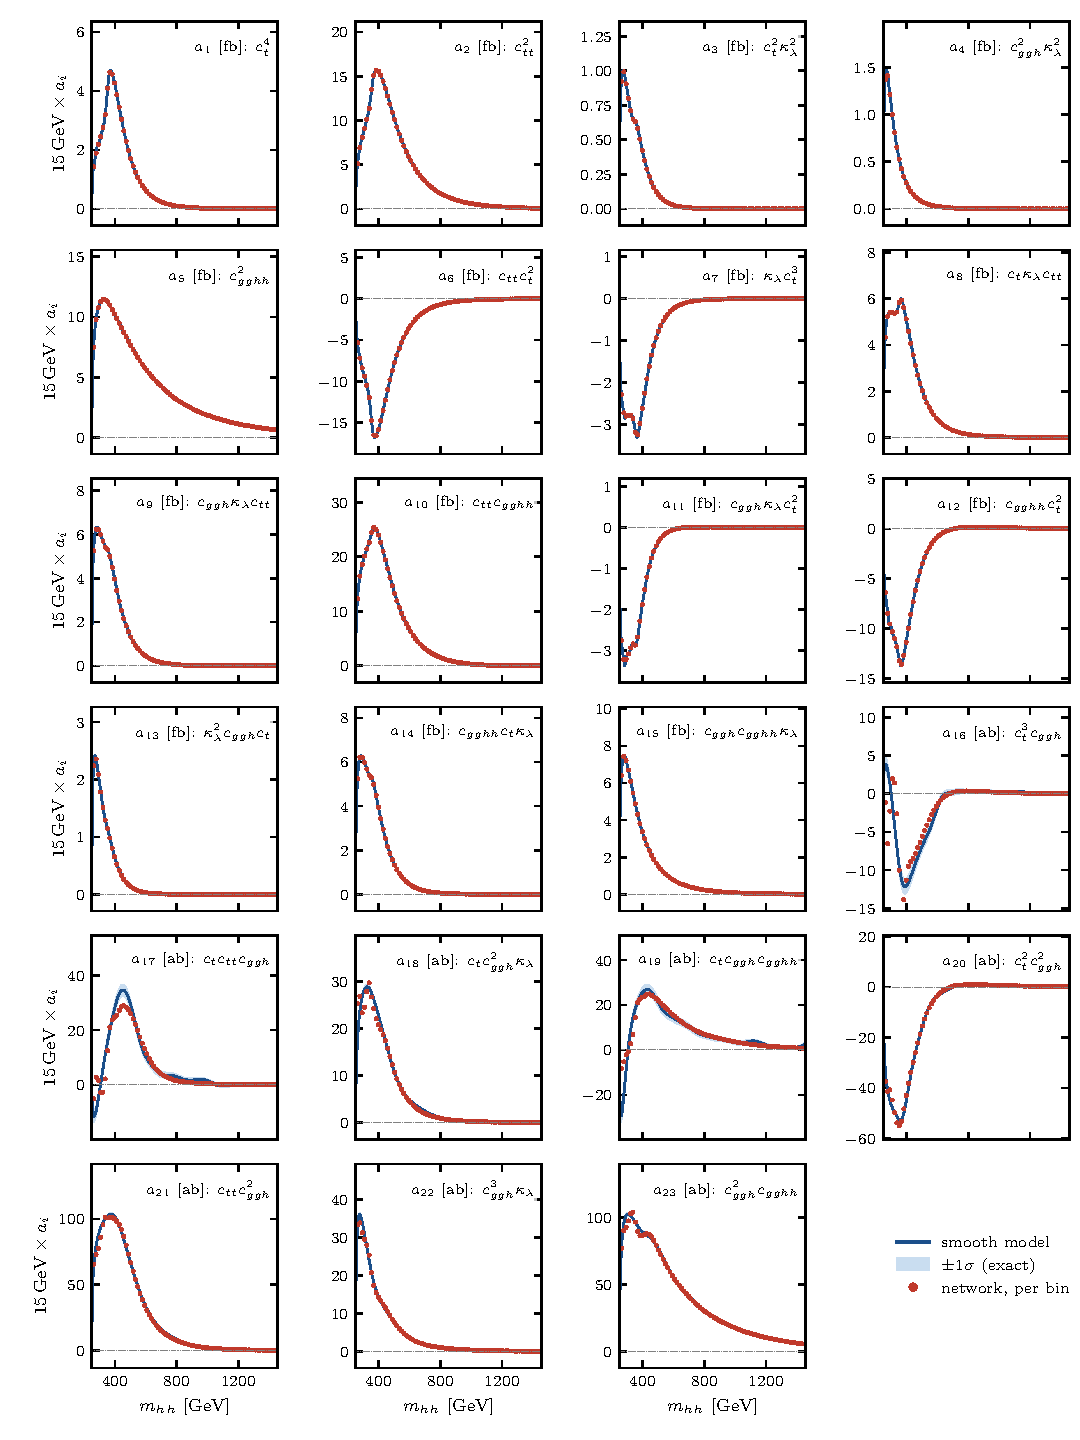
\includegraphics[width=\textwidth]{fig_coefficients.pdf}
\caption{The 23 coefficient functions $a_i(m_{hh})$, the cross section per 15~GeV bin
multiplying the monomial $C_i(\theta)$ shown in each panel, so that
$\sigma = \sum_i C_i(\theta)\,a_i(m_{hh})$. Line: mean of the 20 fine-tuned networks.
Dark band: spread between the networks ($\pm1\sigma$); light band: total network
uncertainty, adding the Laplace uncertainty of each network ($\pm1\sigma$). Units are fb,
or ab for the eight smallest functions. The functions are determined only through the
combinations $\sum_i C_i a_i$ at the sampled HEFT points; functions whose monomials are
small or nearly degenerate over the sample ($a_{16}$--$a_{20}$) are the least well
determined.}
\label{fig:coefficients}
\end{figure}
